\documentclass{article}
\usepackage[margin=1in]{geometry}
\usepackage{amsmath}
\usepackage{graphicx} %insert images
\usepackage{bbm}
\title{Econ899b PS4}
\author{Hiroaki Shirai}
\begin{document}
\maketitle

\begin{enumerate}
\item The expected value function can be written as follows:
  \begin{equation*}
    \begin{split}
      \bar{V} &= E_{\epsilon}[V(i,c,p,\epsilon)] \\
      &= E_{\epsilon}[\max_{a} U(a|i,c,p,\epsilon) + \beta \sum E[V(i',c',p',\epsilon']Pr(c',p'|c,p,a)]] \\
      &= E_{\epsilon}[\max_{a} \mathbbm{1}(a =1)(\alpha c - p) + \mathbbm{1}(a =1)\mathbbm{1}(i > 1)\alpha c + \mathbbm{1}(a =1)\mathbbm{1}(i = 1)\lambda\mathbbm{1}(c>0)+ \epsilon(a)\\
      & \ \ \ \ \ + \beta \sum E[V(i',c',p',\epsilon']Pr(c',p'|c,p,a)]] \\
    \end{split}
  \end{equation*}
  Let $v(a, i, c, p) = \mathbbm{1}(a =1)(\alpha c - p) + \mathbbm{1}(a =1)\mathbbm{1}(i > 1)\alpha c + \mathbbm{1}(a =1)\mathbbm{1}(i = 1)\lambda\mathbbm{1}(c>0)+ \beta \sum E[V(\cdot)]Pr(c',p'|c,p,a)]$. Then,
  \begin{equation*}
    E_{\epsilon}[\max_a v(a, i, c, p) + \epsilon(a)] = \ln(\sum_a \exp(v(\cdot))) + \gamma
  \end{equation*}

  The Table is (1).
  \begin{equation}
    \begin{array}{cccc}
      I & C & P & EV \\
      0 & 0 & 4 & 61.12785224254987 \\
      1 & 0 & 4 & 65.01024882086212 \\
      2 & 0 & 4 & 68.48210863284643 \\
      3 & 0 & 4 & 71.66875693503552 \\
      4 & 0 & 4 & 74.63022715292597 \\
      5 & 0 & 4 & 77.39429444746555 \\
      6 & 0 & 4 & 79.95878691331467 \\
      7 & 0 & 4 & 82.2632871179156 \\
      8 & 0 & 4 & 84.07324859344968 \\
      0 & 1 & 4 & 58.49101865421765 \\
      1 & 1 & 4 & 63.12785224254987 \\
      2 & 1 & 4 & 67.01024882086212 \\
      3 & 1 & 4 & 70.48210863284643 \\
      4 & 1 & 4 & 73.66875693503552 \\
      5 & 1 & 4 & 76.63022715292594 \\
      6 & 1 & 4 & 79.39429444746558 \\
      7 & 1 & 4 & 81.95878691331467 \\
      8 & 1 & 4 & 84.2632871179156 \\
      0 & 0 & 1 & 63.24416119042413 \\
      1 & 0 & 1 & 66.89462073690096 \\
      2 & 0 & 1 & 70.20312375430869 \\
      3 & 0 & 1 & 73.26050214629285 \\
      4 & 0 & 1 & 76.11022495925096 \\
      5 & 0 & 1 & 78.76597733882473 \\
      6 & 0 & 1 & 81.20090619366847 \\
      7 & 0 & 1 & 83.28155981827642 \\
      8 & 0 & 1 & 84.27758186000644 \\
      0 & 1 & 1 & 61.025485862098925 \\
      1 & 1 & 1 & 65.24416119042414 \\
      2 & 1 & 1 & 68.89462073690099 \\
      3 & 1 & 1 & 72.20312375430869 \\
      4 & 1 & 1 & 75.26050214629282 \\
      5 & 1 & 1 & 78.11022495925093 \\
      6 & 1 & 1 & 80.76597733882475 \\
      7 & 1 & 1 & 83.20090619366847 \\
      8 & 1 & 1 & 85.28155981827642 \\
    \end{array}
  \end{equation}

\item The result is (2). The difference between the true an implied is too small.
  \begin{equation}
      \begin{array}{ccccc}
        I & C & P & EV & \hat{EV}\\

        0 & 0 & 4 & 61.12785224254987 & 60.71685415008766 \\
        1 & 0 & 4 & 65.01024882086212 & 64.59361123596021 \\
        2 & 0 & 4 & 68.48210863284643 & 68.05323953115087 \\
        3 & 0 & 4 & 71.66875693503552 & 71.21078777903563 \\
        4 & 0 & 4 & 74.63022715292597 & 74.128187694844 \\
        5 & 0 & 4 & 77.39429444746555 & 76.80253283552119 \\
        6 & 0 & 4 & 79.95878691331467 & 79.20529891994728 \\
        7 & 0 & 4 & 82.2632871179156 & 81.24124984308239 \\
        8 & 0 & 4 & 84.07324859344968 & 82.64595938571622 \\
        0 & 1 & 4 & 58.49101865421765 & 58.0797578508909 \\
        1 & 1 & 4 & 63.12785224254987 & 62.71421645611459 \\
        2 & 1 & 4 & 67.01024882086212 & 66.592322238919 \\
        3 & 1 & 4 & 70.48210863284643 & 70.05278380353798 \\
        4 & 1 & 4 & 73.66875693503552 & 73.2073673946673 \\
        5 & 1 & 4 & 76.63022715292594 & 76.12787686979966 \\
        6 & 1 & 4 & 79.39429444746558 & 78.77931511201233 \\
        7 & 1 & 4 & 81.95878691331467 & 81.06049632164435 \\
        8 & 1 & 4 & 84.2632871179156 & 83.17556592207703 \\
        0 & 0 & 1 & 63.24416119042413 & 62.829230140790884 \\
        1 & 0 & 1 & 66.89462073690096 & 66.46700616878599 \\
        2 & 0 & 1 & 70.20312375430869 & 69.75722184911152 \\
        3 & 0 & 1 & 73.26050214629285 & 72.78251015847485 \\
        4 & 0 & 1 & 76.11022495925096 & 75.56841086673374 \\
        5 & 0 & 1 & 78.76597733882473 & 78.10017998173997 \\
        6 & 0 & 1 & 81.20090619366847 & 80.29875755014329 \\
        7 & 0 & 1 & 83.28155981827642 & 82.06923576093345 \\
        8 & 0 & 1 & 84.27758186000644 & 82.65905072376842 \\
        0 & 1 & 1 & 61.025485862098925 & 60.61447742610977 \\
        1 & 1 & 1 & 65.24416119042414 & 64.82752674093717 \\
        2 & 1 & 1 & 68.89462073690099 & 68.47022110976287 \\
        3 & 1 & 1 & 72.20312375430869 & 71.76423459119239 \\
        4 & 1 & 1 & 75.26050214629282 & 74.78554697997075 \\
        5 & 1 & 1 & 78.11022495925093 & 77.49062843672597 \\
        6 & 1 & 1 & 80.76597733882475 & 80.07072261396762 \\
        7 & 1 & 1 & 83.20090619366847 & 82.28185545507503 \\
        8 & 1 & 1 & 85.28155981827642 & 83.02656430722752 \\
      \end{array}
    \end{equation}

  \item The log-likelihood function is

    $$\sum_{i}a_i \log Pr_i(s) + (1-a_i) \log (1-Pr_i(s))$$

    where $Pr_i(s)$ is the conditional choice probability. 
  \item The loglikihood has the following shape. And, the results are the following: MLE: -4.300628278478276
  NFP: -4.300628278478276. Although these values are not matched with results, the value is relatively similar with the true value. Since MLE and NFP yield the same result, there would be a bug in my code.


    \begin{center}
    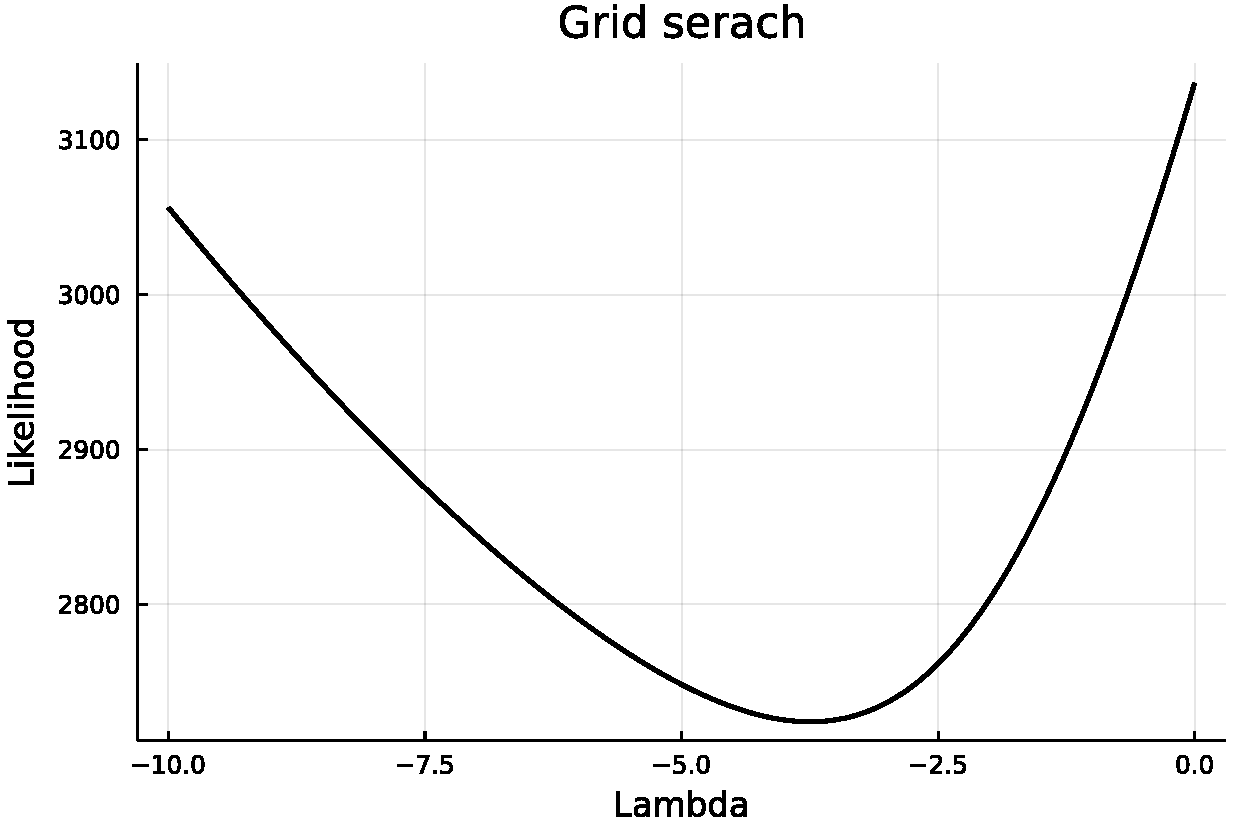
\includegraphics[width = 0.8\textwidth]{./Figures/Q4_grid.pdf}
  \end{center}

\end{enumerate}

\end{document}